% Exact LaTeX recreation of the Airline Reservation System Phase-1 Proposal
% Content aligned with Data Structures and OOP with C++ Syllabus
% Compile with pdfLaTeX. Place member pictures in the same folder if required.

\documentclass[11pt,a4paper]{article}

\usepackage[a4paper,left=2.0cm,right=2.0cm,top=1.55cm,bottom=1.55cm]{geometry}
\usepackage[T1]{fontenc}
\usepackage{lmodern}
\usepackage{graphicx}
\usepackage{xcolor}
\usepackage{array}
\usepackage{tabularx}
\usepackage{ragged2e}
\usepackage{enumitem}
\usepackage{fancyhdr}
\usepackage{tikz}
\usetikzlibrary{arrows.meta,positioning,shapes.geometric}
\usepackage{setspace}
\usepackage{calc}

% -------------------------------------------------
% COLOURS
% -------------------------------------------------
\definecolor{TitleBlue}{RGB}{61,103,154}

% -------------------------------------------------
% GENERAL SETTINGS
% -------------------------------------------------
\setlength{\parindent}{0pt}
\setlength{\parskip}{0pt}
\renewcommand{\arraystretch}{1.0}

\newcommand{\blueheading}[1]{%
    {\sffamily\color{TitleBlue}\fontsize{14}{17}\selectfont #1}%
}

\newcommand{\bluebigheading}[1]{%
    {\sffamily\bfseries\color{TitleBlue}\fontsize{15.5}{18.5}\selectfont #1}%
}

\newcommand{\instruction}[1]{%
    {\itshape\fontsize{10}{12}\selectfont #1}%
}

% -------------------------------------------------
% DYNAMIC NON-OVERFLOWING ANSWER BOX
% Enforces minimum height #1, but automatically expands 
% if inner content exceeds #1 so content never bleeds outside.
% -------------------------------------------------
\newsavebox{\contentbox}
\newcommand{\answerbox}[2][3.0cm]{%
    \vspace{2pt}%
    \noindent
    \sbox{\contentbox}{%
        \begin{minipage}{\dimexpr\textwidth-2\fboxsep-2\fboxrule\relax}
            \vspace{1.5mm}%
            {\fontsize{9.5}{12}\selectfont\itshape #2\par}%
            \vspace{1.5mm}%
        \end{minipage}%
    }%
    \ifdim\dimexpr\ht\contentbox+\dp\contentbox\relax>#1
        \fbox{\usebox{\contentbox}}%
    \else
        \fbox{%
            \begin{minipage}[t][#1][t]{\dimexpr\textwidth-2\fboxsep-2\fboxrule\relax}
                \vspace{1.5mm}%
                {\fontsize{9.5}{12}\selectfont\itshape #2\par}%
                \vfill
            \end{minipage}%
        }%
    \fi
}

% -------------------------------------------------
% HEADER / FOOTER
% -------------------------------------------------
\pagestyle{fancy}
\fancyhf{}
\renewcommand{\headrulewidth}{0pt}
\renewcommand{\footrulewidth}{0pt}

\fancyhead[L]{%
    \sffamily\bfseries\itshape\fontsize{10}{11.5}\selectfont
    DSCPP-III-2026-T351
}
\fancyhead[R]{}
\fancyfoot[R]{%
    \itshape\fontsize{9.5}{11.5}\selectfont
    Page \thepage
}
\setlength{\headheight}{14pt}
\setlength{\headsep}{20pt}
\setlength{\footskip}{20pt}

% -------------------------------------------------
% PAGE 1
% -------------------------------------------------
\begin{document}

\vspace*{2mm}

\bluebigheading{PROJECT AND TEAM INFORMATION}

\vspace{6mm}

\blueheading{Project Title}

\vspace{1mm}

\instruction{}

\answerbox[1.1cm]{AeroSync: An Object-Oriented Airline Reservation and Inventory Management System Utilizing Advanced Data Structures in C++}

\vspace{6mm}

\blueheading{Student / Team Information}

\vspace{2mm}

\noindent
\begin{tabularx}{\textwidth}{|>{\RaggedRight\arraybackslash}p{0.48\textwidth}|>{\RaggedRight\arraybackslash}X|}
\hline
\begin{minipage}[t]{\linewidth}
\vspace{1.5mm}
\textit{Team Name:}\\[-1mm]
\textit{Team \#}
\vspace{1.5mm}
\end{minipage}
&
\begin{minipage}[t]{\linewidth}
\vspace{1.5mm}
\textit{DSCPP-III-2026-T351}\\
\textit{}
\vspace{1.5mm}
\end{minipage}
\\
\hline
\begin{minipage}[t]{\linewidth}
\vspace{2mm}
\textbf{Team member 1 (Team Lead)}\\[1mm]
\textit{(Last Name, name: student ID: email, picture):}
\vspace{2mm}
\end{minipage}
&
\begin{minipage}[t]{\linewidth}
\vspace{2mm}
\textit{Raj, Ashu -- 2510360055}\\
\textit{amu07415@gmail.com}

\vspace{1.5mm}
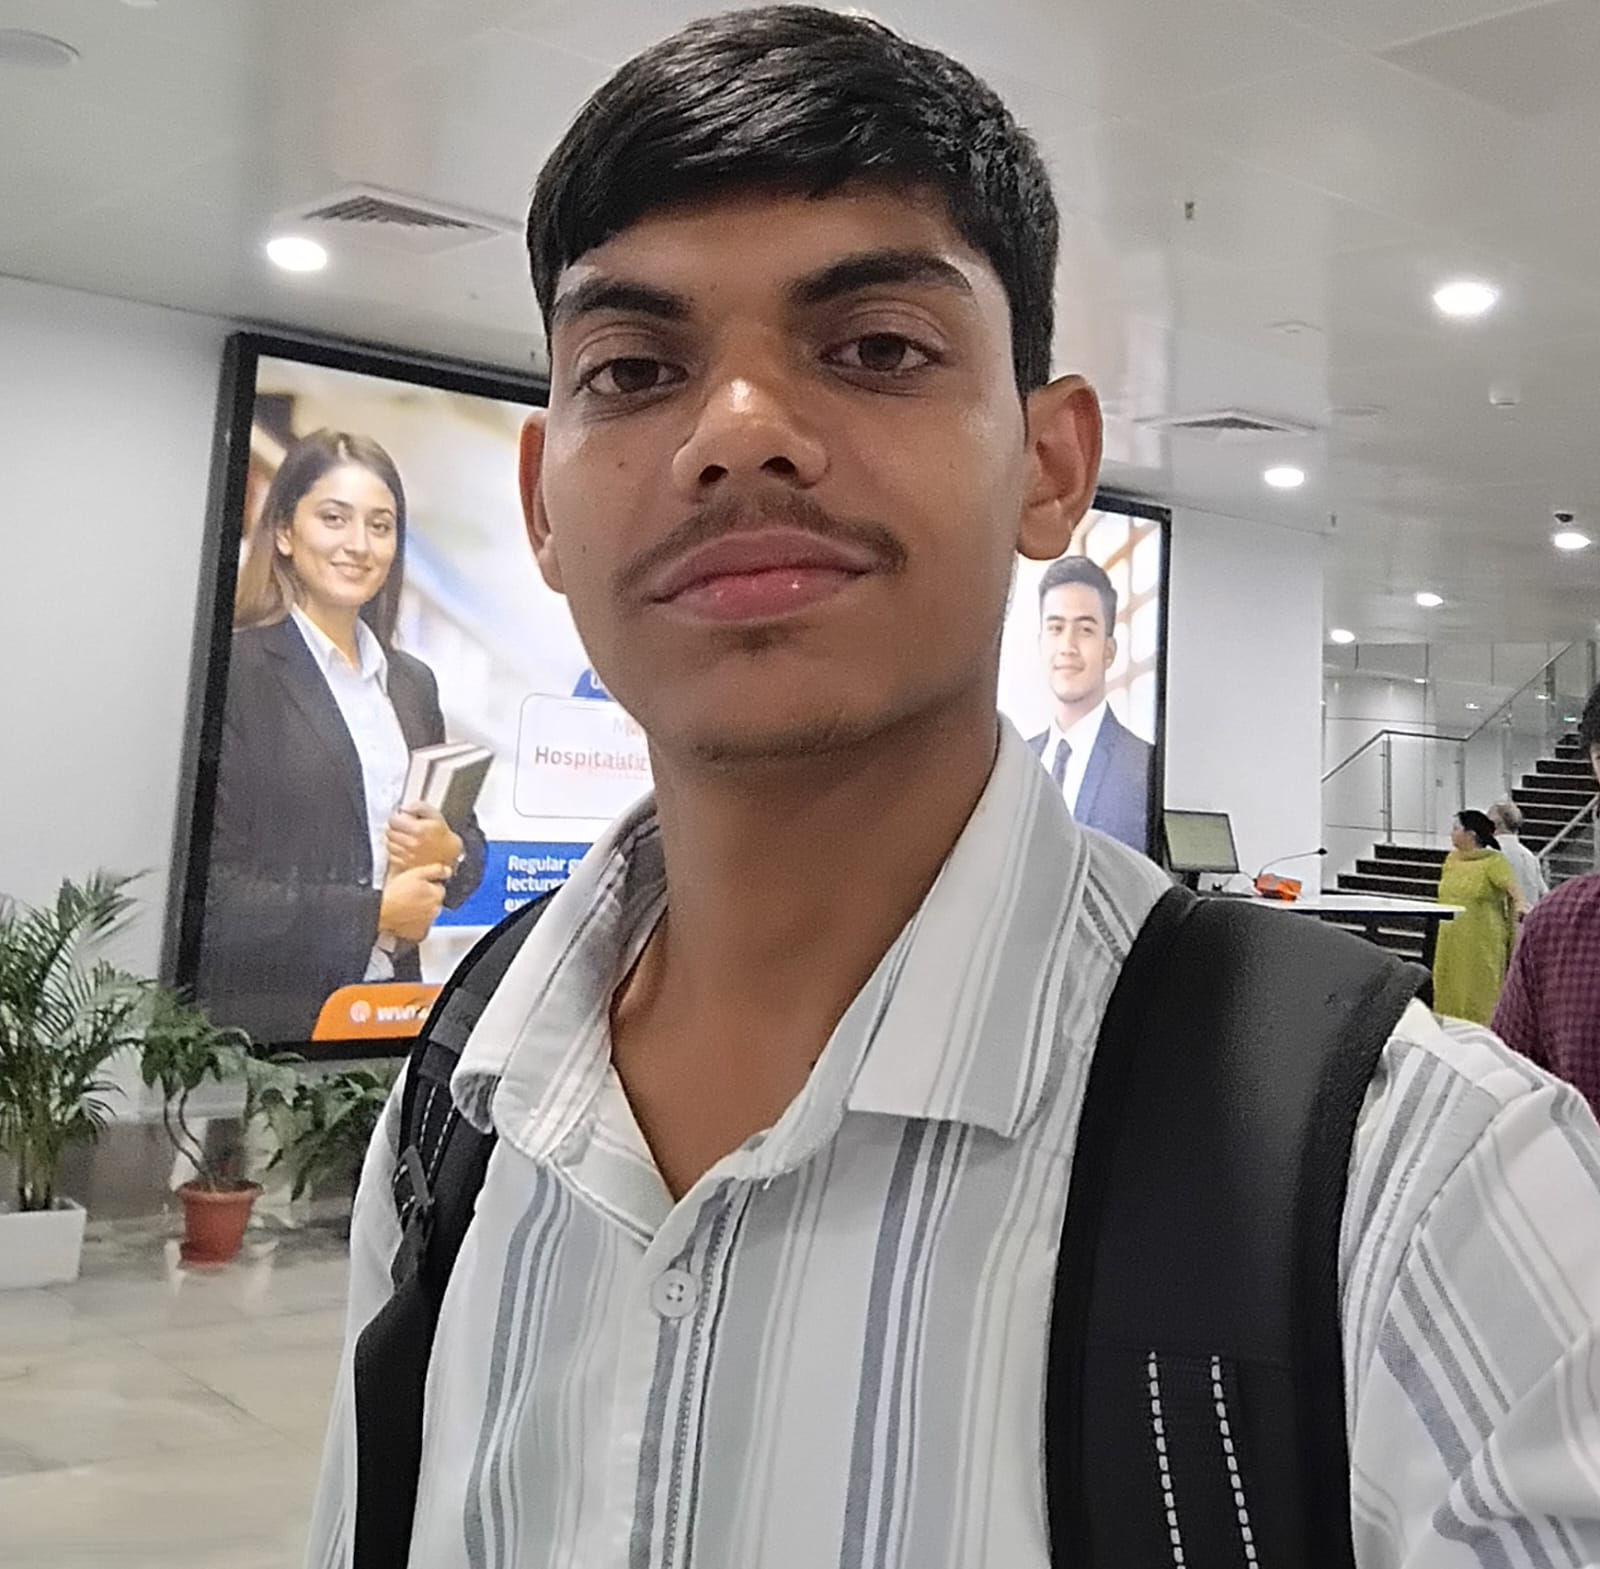
\includegraphics[width=2.5cm,height=1.4cm,keepaspectratio]{member1.png}
\vspace{2mm}
\end{minipage}
\\
\hline
\begin{minipage}[t]{\linewidth}
\vspace{2mm}
\textbf{Team member 2}\\[1mm]
\textit{(Last Name, name: student ID: email, picture):}
\vspace{2mm}
\end{minipage}
&
\begin{minipage}[t]{\linewidth}
\vspace{2mm}
\textit{Airi, Harshit -- 2510011802}\\
\textit{harshit12airi@gmail.com}

\vspace{1.5mm}
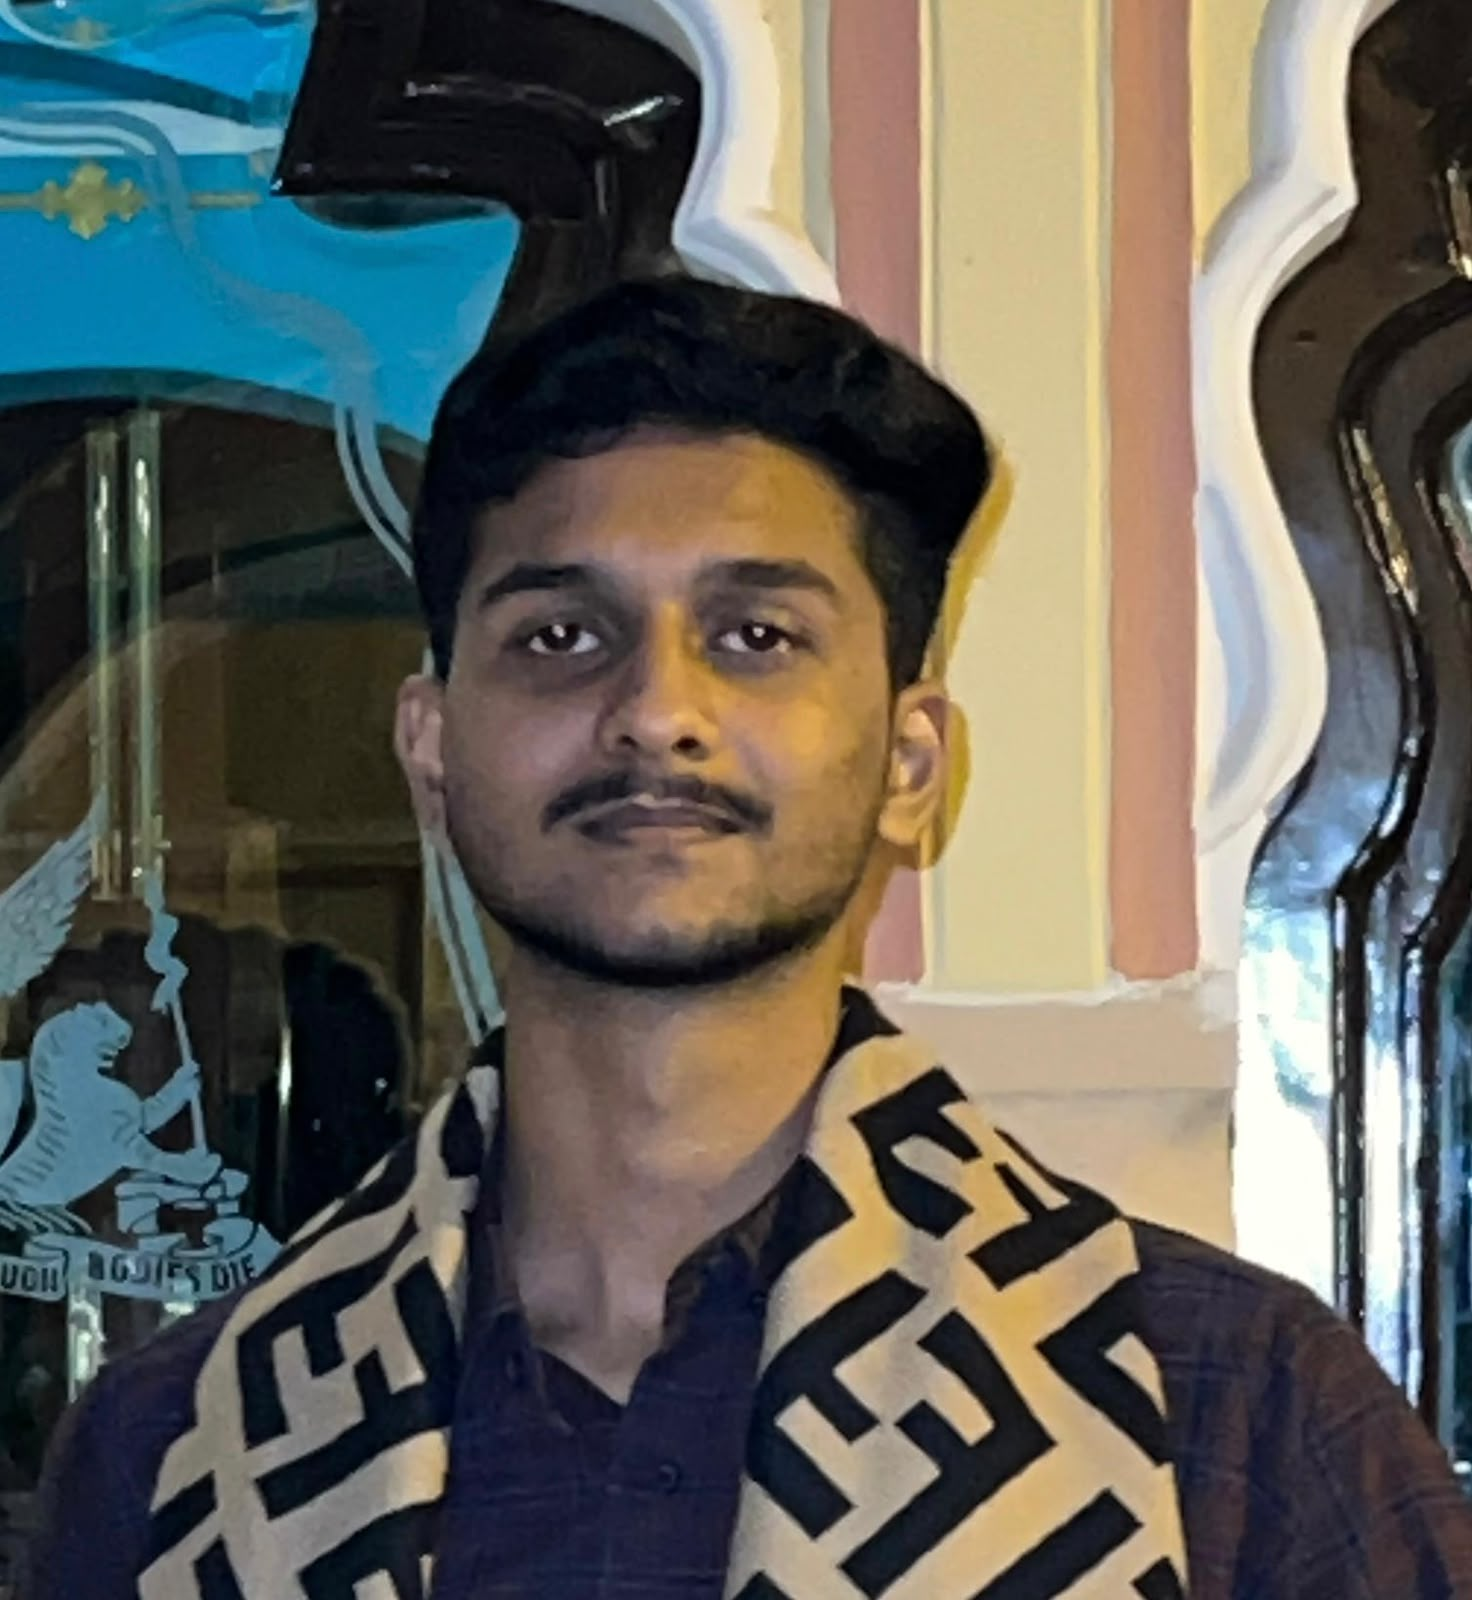
\includegraphics[width=2.5cm,height=1.4cm,keepaspectratio]{member2.png}
\vspace{2mm}
\end{minipage}
\\
\hline
\begin{minipage}[t]{\linewidth}
\vspace{2mm}
\textbf{Team member 3}\\[1mm]
\textit{(Last Name, name: student ID: email, picture):}
\vspace{2mm}
\end{minipage}
&
\begin{minipage}[t]{\linewidth}
\vspace{2mm}
\textit{Pandey, Ayush -- 2510011835}\\
\textit{ayush.pandey@gmail.com}

\vspace{1.5mm}
\includegraphics[width=2.5cm,height=1.4cm,keepaspectratio]{member3.png}
\vspace{2mm}
\end{minipage}
\\
\hline
\end{tabularx}

\newpage

% -------------------------------------------------
% PAGE 2
% -------------------------------------------------

\bluebigheading{PROPOSAL DESCRIPTION}

\vspace{6mm}

\blueheading{Motivation}

\vspace{1mm}

\instruction{}

\answerbox[3.2cm]{Managing airline passenger bookings, seat layouts, and flight schedules requires high algorithmic efficiency, deterministic memory management, and robust data encapsulation. In high-frequency operational environments, arbitrary array allocations lead to high memory fragmentation and inefficient searching. Unorganized waitlists cause fairness violations during seat cancellations. Addressing these issues from foundational computer science principles is vital. By leveraging custom Abstract Data Types (ADTs) in C++---such as two-dimensional arrays for direct row-column cabin addressing, circular queues for bounded FIFO passenger waitlists, priority queues for emergency and VIP boarding, and doubly linked lists for dynamic passenger manifests---this project provides a zero-overhead, memory-safe reservation engine that guarantees optimal asymptotic time complexity without relying on heavy external dependencies.}

\vspace{6mm}

\blueheading{State of the Art / Current solution}

\vspace{1mm}

\instruction{}

\answerbox[2.7cm]{Contemporary airline reservation systems rely heavily on high-level managed runtime languages and multi-tiered relational databases. Although feature-rich, these systems introduce garbage-collection pauses, heavy runtime memory footprints, and high latency overheads during peak transactional spikes. Existing academic implementations often resort to rigid single-dimensional static arrays that waste space ($O(N)$ overhead regardless of passenger load) and lack object-oriented modularity. This project bridges this gap by engineering specialized linear data structures and dynamic object lifecycles in C++, enforcing strict Resource Acquisition Is Initialization (RAII) and precise pointer semantics.}

\vspace{6mm}

\blueheading{Project Goals and Milestones}

\vspace{1mm}

\instruction{}

\answerbox[3.8cm]{The primary objective is to implement a high-performance, console-based Airline Reservation System in C++ integrating custom Abstract Data Types and Object-Oriented Programming mechanisms.
\begin{itemize}[leftmargin=*,noitemsep,topsep=1.5pt]
\item \textbf{Milestone 1 (Weeks 1--3):} Design ADT specifications and class hierarchies (\texttt{Flight}, \texttt{Passenger}, \texttt{SeatMap}); implement 2D array row-major memory mapping for cabin seating.
\item \textbf{Milestone 2 (Weeks 4--6):} Implement dynamic Doubly Linked Lists for passenger manifests and a Stack ADT for multi-level booking transaction undo/rollback operations.
\item \textbf{Milestone 3 (Weeks 7--9):} Construct an array-based Circular Queue for FIFO standby waitlists and a Priority Queue for elite/medical boarding triage.
\item \textbf{Milestone 4 (Weeks 10--12):} Implement operator overloading for ticket fare aggregation and stream I/O, dynamic object destruction to guarantee zero memory leaks, and complexity benchmarking.
\end{itemize}}

\vspace{6mm}

\blueheading{Project Approach}

\vspace{1mm}

\instruction{}

\answerbox[3.0cm]{The system follows a modular C++ Object-Oriented architecture partitioned into distinct ADT layers. The \textbf{Seating Module} utilizes a 2D dynamic array with custom address calculation logic for constant-time $O(1)$ seat assignment. The \textbf{Manifest Module} implements a Doubly Linked List with two-way pointer traversal for linear insertion and deletion of passenger records. The \textbf{Queueing Module} employs a Circular Queue to avoid memory shifts during waitlist dequeuing, supplemented by a Priority Queue for fare-class sorting. The \textbf{Transaction Module} uses an array-based Stack to track booking actions for instant rollback. The core classes encapsulate data members using access specifiers, parameterized/copy constructors, destructors for heap reclamation via \texttt{delete}, and overloaded operators (\texttt{+}, \texttt{<<}, \texttt{>>}) for arithmetic fare summation and formatted stream console output.}

\newpage

% -------------------------------------------------
% PAGE 3
% -------------------------------------------------

\blueheading{System Architecture (High Level Diagram)}

\vspace{1mm}

\instruction{}

\answerbox[4.2cm]{%
\centering
\vspace{1mm}
\resizebox{!}{3.3cm}{%
\begin{tikzpicture}[
    node distance=0.8cm and 0.8cm,
    font=\sffamily\scriptsize,
    box/.style={draw=TitleBlue, thick, rounded corners=3pt, align=center, fill=white, inner sep=3.5pt, minimum height=0.75cm},
    service/.style={draw=TitleBlue!80, fill=TitleBlue!10, rounded corners=3pt, align=center, inner sep=3.5pt, text width=2.4cm, minimum height=0.75cm},
    db/.style={rectangle, dashed, draw=TitleBlue, fill=TitleBlue!15, rounded corners=2pt, align=center, inner sep=2.5pt, text width=1.8cm, minimum height=0.75cm},
    arrow/.style={-{Latex[scale=0.75]}, thick, color=TitleBlue}
]
    % Nodes
    \node[box, text width=2.2cm] (client) {Client I/O Interface\\(Overloaded \texttt{<<}, \texttt{>>})};
    \node[box, right=0.7cm of client, text width=2.1cm] (gateway) {Reservation Manager\\(C++ Class \& Pointers)};
    
    % ADT Modules
    \node[service, right=0.8cm of gateway, yshift=1.25cm] (seatmap) {Cabin Seat Matrix\\(2D Dynamic Array)};
    \node[service, right=0.8cm of gateway, yshift=0.0cm] (manifest) {Passenger Manifest\\(Doubly Linked List)};
    \node[service, right=0.8cm of gateway, yshift=-1.25cm] (queue) {Waitlist \& Boarding\\(Circular / Priority Q)};

    % Specialized Modules
    \node[db, right=0.8cm of seatmap] (stack) {Booking History\\(Stack ADT / Undo)};
    \node[db, right=0.8cm of manifest] (filestore) {Persistent Storage\\(File I/O Streams)};
    \node[box, right=0.8cm of queue, text width=1.9cm] (overload) {Billing Engine\\(Operator \texttt{+} / \texttt{-})};

    % Connections
    \draw[arrow] (client) -- node[above, font=\tiny]{Method Call} (gateway);
    \draw[arrow] (gateway) |- (seatmap);
    \draw[arrow] (gateway) -- (manifest);
    \draw[arrow] (gateway) |- (queue);

    \draw[arrow] (seatmap) -- (stack);
    \draw[arrow] (manifest) -- (filestore);
    \draw[arrow] (manifest) to[out=35,in=-145] (stack);
    \draw[arrow] (queue) -- (overload);
\end{tikzpicture}
}
}

\vspace{5mm}

\blueheading{Project Outcome / Deliverables}

\vspace{1mm}

\instruction{}

\answerbox[3.2cm]{%
\begin{itemize}[leftmargin=*,noitemsep,topsep=1pt]
\item \textbf{C++ Reservation Application:} Fully functional executable demonstrating robust memory management, zero leaks, and interactive terminal workflows.
\item \textbf{Custom ADT Library:} Clean, modular implementations of 2D Seat Array, Circular Queue, Priority Queue, Doubly Linked List, and Transaction Stack.
\item \textbf{OOP Implementation Suite:} Validated use of constructors/destructors, static data members for passenger ID generation, friend functions, and overloaded operators.
\item \textbf{Complexity Benchmark Document:} Detailed theoretical vs. empirical execution report measuring time-space trade-offs across all core ADT operations.
\end{itemize}}

\vspace{5mm}

\blueheading{Assumptions}

\vspace{1mm}

\instruction{}

\answerbox[2.1cm]{System execution is localized to single-process sequential execution in C++. Maximum cabin dimensions and base flight capacities are specified via compile-time constants or initial configuration parameters. Memory allocation via the \texttt{new} operator is assumed to operate within normal operating system heap limits without unexpected bad allocations. User terminal input follows valid alphanumeric character sets.}

\vspace{5mm}

\blueheading{References}

\vspace{1mm}

\instruction{}

\answerbox[2.4cm]{%
\begin{itemize}[leftmargin=*,noitemsep,topsep=1pt]
\item Horowitz, E., Sahni, S., and Anderson-Freed, S., \textit{Fundamentals of Data Structures in C}, 2nd Ed., Silicon Press, 2008.
\item Stroustrup, B., \textit{The C++ Programming Language}, 4th Ed., Addison-Wesley, 2013.
\item Lippman, S. B., Lajoie, J., and Moo, B. E., \textit{C++ Primer}, 5th Ed., Addison-Wesley Professional, 2012.
\end{itemize}}

\end{document}